\documentclass{article}
\usepackage[margin=1in]{geometry}
\usepackage{enumitem}
\usepackage{setspace}
\usepackage{amsmath}
\usepackage{amssymb}
\usepackage{physics}
\usepackage{relsize}
\usepackage{graphicx}

\title{Math 132 Homework 8}
\date{11/29/2020}
\author{Jiaping Zeng}

\begin{document}
\setstretch{1.35}
\maketitle


\noindent Proposition ($\bigstar$). Suppose $f(z)$ and $g(z)$ are analytic at $z_0$. If $f(z)$ has a zero of order $n$ at $z_0$ (or letting $n=0$ if $f(z_0)\neq 0$) and $g(z)$ has a zero of order $m$ at $z_0$, then \[h(z)=\dfrac{f(z)}{g(z)}\text{ has }\begin{cases}
            \text{a removable singularity at }z_0     & \text{if }m\leq n; \\
            \text{a pole of order }m-n\text{ at }z_0, & \text{if }m>n.
      \end{cases}\]
\begin{itemize}
      \item [4.6.1] $(1-z^2)\sin z$\\
            \textbf{Answer}: We have $(1-z^2)\sin z=(1+z)(1-z)\sin z$, so the isolated zeros are at $-1,1$ and $k\pi,k\in\mathbb{Z}$. The zeroes $-1$ and $1$ have order 1; the zeroes of $\sin z$ also have order 1 as shown in class.
      \item [4.6.2] $z^3(e^z-1)$\\
            \textbf{Answer}: Since $z^3=0$ when $z=0$ and $e^z-1=0$ when $z=2k\pi i,k\in\mathbb{Z}$, the isolated zeroes are at $0$ and $2k\pi i,k\in\mathbb{Z}$. Let $f(z)=z^3$, then $f'''(0)=6\neq 0$, so $z_0=0$ is a zero of order 3. Now let $g(z)=e^z-1$, then $g'(0)=e^0=1\neq 0$, so $z_0=2k\pi i,k\neq 0\in\mathbb{Z}$ are zeroes of order 1.
      \item [4.6.9] $1-\dfrac{z^2}{2}-\cos z$\\
            \textbf{Answer}: Let $f(z)=1-\dfrac{z^2}{2}-\cos z$, then we have $f'(z)=\sin z-z$, $f''(z)=\cos z-1$, $f'''(z)=-\sin z$ and $f^{(4)}(z)=-\cos z$. By substituting $z_0=0$, we have $f(0)=0$, $f'(0)=0$, $f''(0)=0$, $f'''(0)=0$ and $f^{(4)}=-1\neq 0$, so $z_0=0$ is a zero of order 4.
      \item [4.6.11] $z-\sin z$\\
            \textbf{Answer}: Let $f(z)=z-\sin z$, then we have $f'(z)=1-\cos z$, $f''(z)=\sin z$ and $f'''(z)=\cos z$. By substituting $z_0=0$, we have $f(0)=0$, $f'(0)=0$, $f''(0)=0$ and $f'''(0)=1\neq 0$, so $z_0=0$ is a zero of order 3.
      \item [4.6.15] $\dfrac{z(z-1)^2}{\sin(\pi z)\sin z}$\\
            \textbf{Answer}: Let $f(z)=z(z-1)^2$, $g(z)=\sin(\pi z)\sin z$ and $h(z)=\dfrac{z(z-1)^2}{\sin(\pi z)\sin z}=\dfrac{f(z)}{g(z)}$. Then $f(z)$ has a zero of order 1 at $z_0=0$ and another zero of order 2 at $z_0=1$; in addition, since $\sin(k\pi)=0$ for $k\in\mathbb{Z}$, $g(z)$ has zeroes at $z_0=k$ and $z_0=k\pi,k\in\mathbb{Z}$. Since $g(0)=g'(0)=0$ and $g''(0)\neq 0$, we have a zero of order 2 at $z_0=0$. The other zeroes $z_0=k$ and $z_0=k\pi,k\neq 0\in\mathbb{Z}$ are order 1 as $g'(z_0)\neq 0$ there.\\
            Using Proposition $\bigstar$, we have $n=1$ and $m=2$ at $z_0=0$, so $h(z)$ has a pole of order 1 at $z_0=0$. Since $\lim_{z\rightarrow 1}h(z)=0$, we can define $\tilde{h}(1)=0$ to make $\tilde{h}(z)$ analytic. At $z_0=1$, we have $n=2$ and $m=1$, so $h(z)$ has a removable singularity at $z_0=1$. At zeroes $z_0=k$ and $z_0=k\pi,k\neq 0,1\in\mathbb{Z}$, we have $n=0$ and $m=1$, so $h(z)$ has poles of order 1 there.
      \item [4.6.16] $e^\frac{1}{1-z}+\dfrac{1}{1-z}$\\
            \textbf{Answer}: By taylor expansion we have $e^\frac{1}{1-z}=1+\dfrac{1}{1-z}+\dfrac{1}{2(1-z)^2}+\dfrac{1}{3!(1-z)^3}+\ldots$, so $e^\frac{1}{1-z}+\dfrac{1}{1-z}=1+\dfrac{2}{1-z}+\dfrac{1}{2(1-z)^2}+\dfrac{1}{3!(1-z)^3}+\ldots$. Therefore there is an essential singularity at $0$.
      \item [4.6.18] $\dfrac{z}{e^z-1}$\\
            \textbf{Answer}: Let $f(z)=z$, $g(z)=e^z-1$ and $h(z)=\dfrac{z}{e^z-1}=\dfrac{f(z)}{g(z)}$. Then $f(z)$ has a zero of order 1 at $z_0=0$ and $g(z)$ has zeroes of order 1 (shown in 4.6.2) at $z_0=2k\pi i,k\in\mathbb{Z}$.\\
            Using Proposition $\bigstar$, we have $n=1$ and $m=1$ at $z_0=0$, so $h(z)$ has a removable singularity at $z_0=0$. Since $\lim_{z\rightarrow 0}h(z)=1$, we can define $\tilde{h}(0)=1$ to make $\tilde{h}(z)$ analytic. At $z_0=2k\pi i,k\neq 0\in\mathbb{Z}$, we have $n=0$ and $m=1$, so $h(z)$ has poles of order 1 at those singularities.
      \item [P1] Use the argument principle to find the number of zeros of \[f(z)=z^5+z^4+13z^3+10\] in the first quadrant.\\
            \textbf{Answer}: Let $R$ be sufficiently large such that all zeroes of $f(z)$ is enclosed by the curve $\gamma_R=[[0,R],\sigma_R,[iR,0]]$ as shown below.
            \begin{center}
                  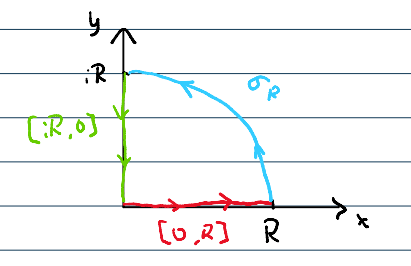
\includegraphics[width=3in]{p1-1.png}
            \end{center}
            Then,
            \begin{itemize}
                  \item [1.] $f([0,R])$: $f(x)=x^5+x^4+13x^3+10$ for $x\in[0,R]$
                  \item [2.] $f(\sigma_R)$: $f(Re^{it})=R^5e^{5it}+R^4e^{4it}+13R^3e^{3it}+10\approx R^5e^{5it}$ for $t\in[0,\frac{\pi}{2}]$
                  \item [3.] $f([iR,0]): f(iy)=iy^5+y^4-13iy^3+10=(y^4+10)+(y^5-13y^3)i$ for $y\in[0,R]$
            \end{itemize}
            Note that $f(z)\neq 0$ on $\gamma_R$ as
            \begin{itemize}
                  \item [1.] $f(z)\geq 10$ on $[0,R]$
                  \item [2.] $R$ was chosen sufficiently large such that $f(z)\neq 0$ on $\sigma_R$
                  \item [3.] $f(iy)=(y^4+10)+(y^5-13y^3)i=(y^4+10)+y^3(y-\sqrt{13})(y+\sqrt{13})i\implies\Re f(iy)$ and $\Im f(iy)$ have no common zeroes $\implies f(z)\neq 0$ on $[iR,0]$
            \end{itemize}
            Now we can sketch $f(\gamma_R)$. Since $f(x)$ for $x\in[0,R]$ always returns a real value, $[0,R]$ maps to $[10,N_1]$ on the real axis where $N_1$ is some large number. Then, since $f(iR)=(R^4+10)+(R^5-13R^3)i\approx R^4+R^5i\approx R^5i$, we also know that $\sigma_R$ ends at some point in the first quadrant, close to the positive imaginary axis. Then since $f(Re^{it})\approx R^5e^{i(5t)},t\in[0,\frac{\pi}{2}]\implies 5t\in[0,\frac{5\pi}{2}]$, $\sigma_R$ is mapped to a circular path that wraps around the origin once and ends near the positive imaginary axis as shown below.
            \begin{center}
                  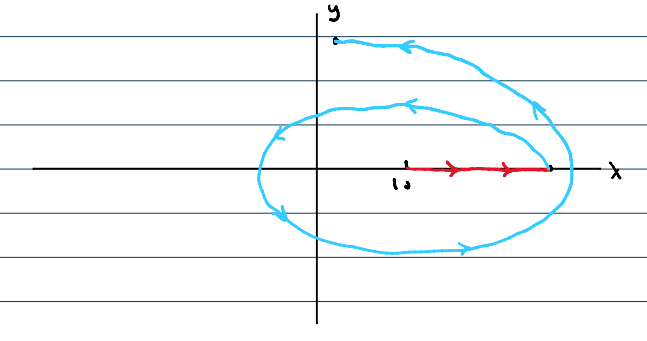
\includegraphics[width=3in]{p1-2.png}
            \end{center}
            Now we can use a sign chart to find the map of $[iR,0]$:
            \begin{center}
                  \begin{tabular}{c|c|c}
                        \hline
                        $y=$          & $(0,\sqrt{13})$ & $(\sqrt{13},R)$ \\
                        \hline\hline
                        Quadrant      & IV              & I               \\
                        \hline\hline
                        $\Re f(iy)$   & +               & +               \\
                        \hline
                        $y^4+10$      & +               & +               \\
                        \hline\hline
                        $\Im f(iy)$   & -               & +               \\
                        \hline
                        $y^3$         & +               & +               \\
                        \hline
                        $y-\sqrt{13}$ & -               & +               \\
                        \hline
                        $y+\sqrt{13}$ & +               & +               \\
                        \hline\hline
                  \end{tabular}
            \end{center}
            Then our $f(\gamma_R)$ looks like:
            \begin{center}
                  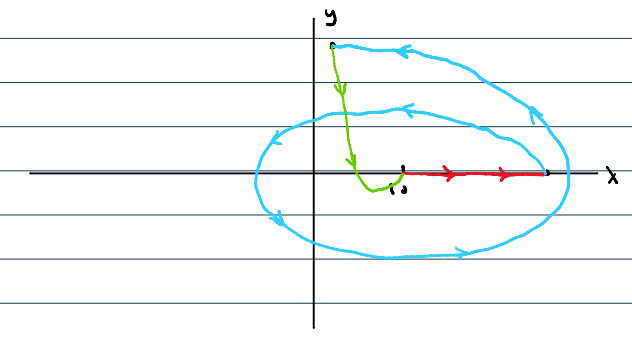
\includegraphics[width=3in]{p1-3.png}
            \end{center}
            So by the argument principle, since $f(\gamma_R)$ wraps counterclockwise around the origin once, we have $N_0-N_\infty=1$. Since $f(z)$ is analytic, then $f(z)$ has no poles $\implies N_\infty=0$. Therefore $N_0=1\implies f(z)$ has one zero in the first quadrant.
      \item [P2] Use the argument principle to find the number of zeros of \[f(z)=z^4+z^3+10z^2+4z+9\] in the first quadrant.\\
            \textbf{Answer}: Let $R$ be sufficiently large such that all zeroes of $f(z)$ is enclosed by the curve $\gamma_R=[[0,R],\sigma_R,[iR,0]]$ as shown below.
            \begin{center}
                  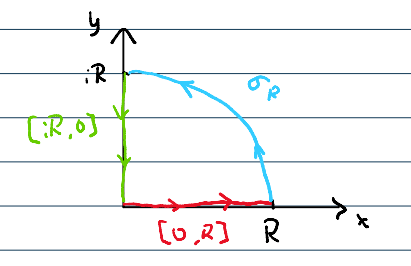
\includegraphics[width=3in]{p2-1.png}
            \end{center}
            Then,
            \begin{itemize}
                  \item [1.] $f([0,R])$: $f(x)=x^4+x^3+10x^2+4x+9$ for $x\in[0,R]$
                  \item [2.] $f(\sigma_R)$: $f(Re^{it})=R^4e^{4it}+R^3e^{3it}+10R^2e^{2it}+4Re^{it}+9\approx R^4e^{4it}$ for $t\in[0,\frac{\pi}{2}]$
                  \item [3.] $f([iR,0]): f(iy)=y^4-iy^3-10y^2+4iy+9=(y^4-10y^2+9)+(-y^3+4y)i$ for $y\in[0,R]$
            \end{itemize}
            Note that $f(z)\neq 0$ on $\gamma_R$ as
            \begin{itemize}
                  \item [1.] $f(z)\geq 9$ on $[0,R]$
                  \item [2.] $R$ was chosen sufficiently large such that $f(z)\neq 0$ on $\sigma_R$
                  \item [3.] $f(iy)=(y^4-10y^2+9)+(-y^3+4y)i=(y-3)(y-1)(y+1)(y+3)-y(y-2)(y+2)i\implies\Re f(iy)$ and $\Im f(iy)$ have no common zeroes $\implies f(z)\neq 0$ on $[iR,0]$
            \end{itemize}
            Now we can sketch $f(\gamma_R)$. Since $f(x)$ for $x\in[0,R]$ always returns a real value, $[0,R]$ maps to $[9,N_1]$ on the real axis where $N_1$ is some large number. Then, since $f(iR)=(R^4-10R^2+9)+(-R^3+4R)i\approx R^4-R^3i\approx R^4$, we also know that $\gamma_R$ ends at some point in the fourth quadrant, close to the positive real axis. Then since $f(Re^{it})\approx R^5e^{i(4t)},t\in[0,\frac{\pi}{2}]\implies 4t\in[0,2\pi]$, $\sigma_R$ is mapped to a circular path that wraps around the origin once and ends near the positive real axis as shown below.
            \begin{center}
                  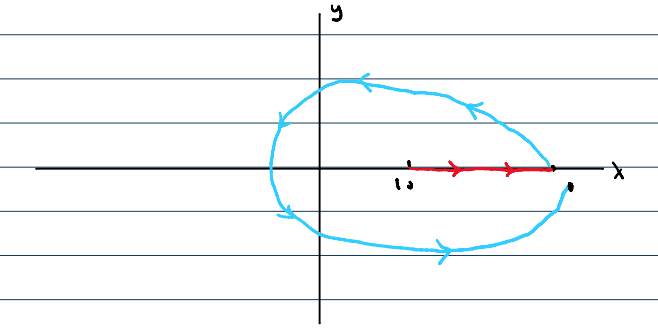
\includegraphics[width=3in]{p2-2.png}
            \end{center}
            Now we can use a sign chart to find the map of $[iR,0]$:
            \begin{center}
                  \begin{tabular}{c|c|c|c|c}
                        \hline
                        $y=$        & $(0,1)$ & $(1,2)$ & $(2,3)$ & $(3,R)$ \\
                        \hline\hline
                        Quadrant    & I       & II      & III     & IV      \\
                        \hline\hline
                        $\Re f(iy)$ & +       & -       & -       & +       \\
                        \hline
                        $y-3$       & -       & -       & -       & +       \\
                        \hline
                        $y-1$       & -       & +       & +       & +       \\
                        \hline
                        $y+1$       & +       & +       & +       & +       \\
                        \hline
                        $y+3$       & +       & +       & +       & +       \\
                        \hline\hline
                        $\Im f(iy)$ & +       & +       & -       & -       \\
                        \hline
                        $-y$        & -       & -       & -       & -       \\
                        \hline
                        $y-2$       & -       & -       & +       & +       \\
                        \hline
                        $y+2$       & +       & +       & +       & +       \\
                        \hline\hline
                  \end{tabular}
            \end{center}
            Then our $f(\gamma_R)$ looks like:
            \begin{center}
                  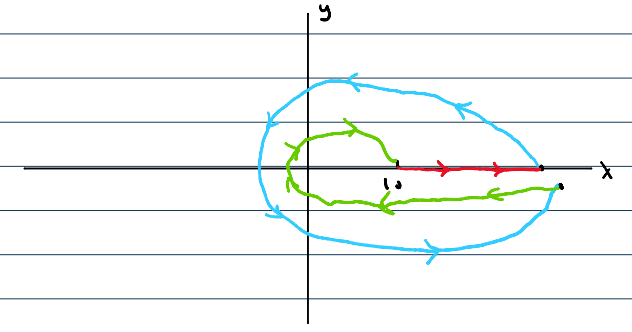
\includegraphics[width=3in]{p2-3.png}
            \end{center}
            So by the argument principle, since $f(\gamma_R)$ wraps counterclockwise around the origin zero times, we have $N_0-N_\infty=0$. Since $f(z)$ is analytic, then $f(z)$ has no poles $\implies N_\infty=0$. Therefore $N_0=0\implies f(z)$ has no zero in the first quadrant.
      \item [P3] Suppose $f(z)$ is analytic at $z_0$ with $f(z_0)\neq 0$, and fix some positive integer $n$. Show that $\dfrac{f(z)}{(z-z_0)^n}$ has a pole of order $n$ at $z_0$.\\
            \textbf{Answer}: Since $f(z)$ is analytic at $z_0$, it has a power series $f(z)=f(z_0)+f'(z_0)(z-z_0)+\dfrac{f''(z_0)}{2}(z-z_0)^2+\ldots$ in $B_r(z_0)$. Then by substitution we have $\dfrac{f(z)}{(z-z_0)^n}=\dfrac{f(z_0)}{(z-z_0)^n}+\dfrac{f'(z_0)}{(z-z_0)^{n-1}}+\ldots$. Since the lowest power term is degree $-n$, by definition $\dfrac{f(z)}{(z-z_0)^n}$ has a pole of order $n$ at $z_0$ by definition.
      \item [P4] Prove Proposition $\bigstar$ above.\\
            \textbf{Answer}: Since $f(z)$ has a zero of order $n$ at $z_0$, we have $f(z)=(z-z_0)^n\tilde{f}(z)$ where $\tilde{f}(z)$ is defined and analytic in some neighborhood of $z_0$ with $\tilde{f}(z_0)\neq 0$. Similarly, we have $g(z)=(z-z_0)^m\tilde{g}(z)$. Then $h(z)=\dfrac{f(z)}{g(z)}=(z-z_0)^{n-m}\dfrac{\tilde{f}(z)}{\tilde{g}(z)}$, where $\dfrac{\tilde{f}(z)}{\tilde{g}(z)}$ is analytic and nonzero at $z_0$.\\
            Then $m\leq n\implies n-m\geq 0$. Then $\lim_{z\rightarrow z_0}\dfrac{f(z)}{g(z)}=\dfrac{\lim_{z\rightarrow z_0}f(z)}{\lim_{z\rightarrow z_0}g(z)}$ by limit laws, which is finite and is therefore a removable singularity.\\
            If $m>n$, then $\tilde{h}(z)=\dfrac{\tilde{f}(z)}{\tilde{g}(z)}$ is analytic in $B_r(z_0)$ for some $r$. Then since $\tilde{h}(z_0)\neq 0$ and $h(z)=\dfrac{\tilde{h}(z)}{(z-z_0)^{m-n}}$, by P3, $h(z)$ has a pole of order $m-n$ at $z_0$.
\end{itemize}
\end{document}